\documentclass[1p]{elsarticle_modified}
%\bibliographystyle{elsarticle-num}

%\usepackage[colorlinks]{hyperref}
%\usepackage{abbrmath_seonhwa} %\Abb, \Ascr, \Acal ,\Abf, \Afrak
\usepackage{amsfonts}
\usepackage{amssymb}
\usepackage{amsmath}
\usepackage{amsthm}
\usepackage{scalefnt}
\usepackage{amsbsy}
\usepackage{kotex}
\usepackage{caption}
\usepackage{subfig}
\usepackage{color}
\usepackage{graphicx}
\usepackage{xcolor} %% white, black, red, green, blue, cyan, magenta, yellow
\usepackage{float}
\usepackage{setspace}
\usepackage{hyperref}

\usepackage{tikz}
\usetikzlibrary{arrows}

\usepackage{multirow}
\usepackage{array} % fixed length table
\usepackage{hhline}

%%%%%%%%%%%%%%%%%%%%%
\makeatletter
\renewcommand*\env@matrix[1][\arraystretch]{%
	\edef\arraystretch{#1}%
	\hskip -\arraycolsep
	\let\@ifnextchar\new@ifnextchar
	\array{*\c@MaxMatrixCols c}}
\makeatother %https://tex.stackexchange.com/questions/14071/how-can-i-increase-the-line-spacing-in-a-matrix
%%%%%%%%%%%%%%%

\usepackage[normalem]{ulem}

\newcommand{\msout}[1]{\ifmmode\text{\sout{\ensuremath{#1}}}\else\sout{#1}\fi}
%SOURCE: \msout is \stkout macro in https://tex.stackexchange.com/questions/20609/strikeout-in-math-mode

\newcommand{\cancel}[1]{
	\ifmmode
	{\color{red}\msout{#1}}
	\else
	{\color{red}\sout{#1}}
	\fi
}

\newcommand{\add}[1]{
	{\color{blue}\uwave{#1}}
}

\newcommand{\replace}[2]{
	\ifmmode
	{\color{red}\msout{#1}}{\color{blue}\uwave{#2}}
	\else
	{\color{red}\sout{#1}}{\color{blue}\uwave{#2}}
	\fi
}

\newcommand{\Sol}{\mathcal{S}} %segment
\newcommand{\D}{D} %diagram
\newcommand{\A}{\mathcal{A}} %arc


%%%%%%%%%%%%%%%%%%%%%%%%%%%%%5 test

\def\sl{\operatorname{\textup{SL}}(2,\Cbb)}
\def\psl{\operatorname{\textup{PSL}}(2,\Cbb)}
\def\quan{\mkern 1mu \triangleright \mkern 1mu}

\theoremstyle{definition}
\newtheorem{thm}{Theorem}[section]
\newtheorem{prop}[thm]{Proposition}
\newtheorem{lem}[thm]{Lemma}
\newtheorem{ques}[thm]{Question}
\newtheorem{cor}[thm]{Corollary}
\newtheorem{defn}[thm]{Definition}
\newtheorem{exam}[thm]{Example}
\newtheorem{rmk}[thm]{Remark}
\newtheorem{alg}[thm]{Algorithm}

\newcommand{\I}{\sqrt{-1}}
\begin{document}

%\begin{frontmatter}
%
%\title{Boundary parabolic representations of knots up to 8 crossings}
%
%%% Group authors per affiliation:
%\author{Yunhi Cho} 
%\address{Department of Mathematics, University of Seoul, Seoul, Korea}
%\ead{yhcho@uos.ac.kr}
%
%
%\author{Seonhwa Kim} %\fnref{s_kim}}
%\address{Center for Geometry and Physics, Institute for Basic Science, Pohang, 37673, Korea}
%\ead{ryeona17@ibs.re.kr}
%
%\author{Hyuk Kim}
%\address{Department of Mathematical Sciences, Seoul National University, Seoul 08826, Korea}
%\ead{hyukkim@snu.ac.kr}
%
%\author{Seokbeom Yoon}
%\address{Department of Mathematical Sciences, Seoul National University, Seoul, 08826,  Korea}
%\ead{sbyoon15@snu.ac.kr}
%
%\begin{abstract}
%We find all boundary parabolic representation of knots up to 8 crossings.
%
%\end{abstract}
%\begin{keyword}
%    \MSC[2010] 57M25 
%\end{keyword}
%
%\end{frontmatter}

%\linenumbers
%\tableofcontents
%
\newcommand\colored[1]{\textcolor{white}{\rule[-0.35ex]{0.8em}{1.4ex}}\kern-0.8em\color{red} #1}%
%\newcommand\colored[1]{\textcolor{white}{ #1}\kern-2.17ex	\textcolor{white}{ #1}\kern-1.81ex	\textcolor{white}{ #1}\kern-2.15ex\color{red}#1	}

{\Large $\underline{12n_{0364}~(K12n_{0364})}$}

\setlength{\tabcolsep}{10pt}
\renewcommand{\arraystretch}{1.6}
\vspace{1cm}\begin{tabular}{m{100pt}>{\centering\arraybackslash}m{274pt}}
\multirow{5}{120pt}{
	\centering
	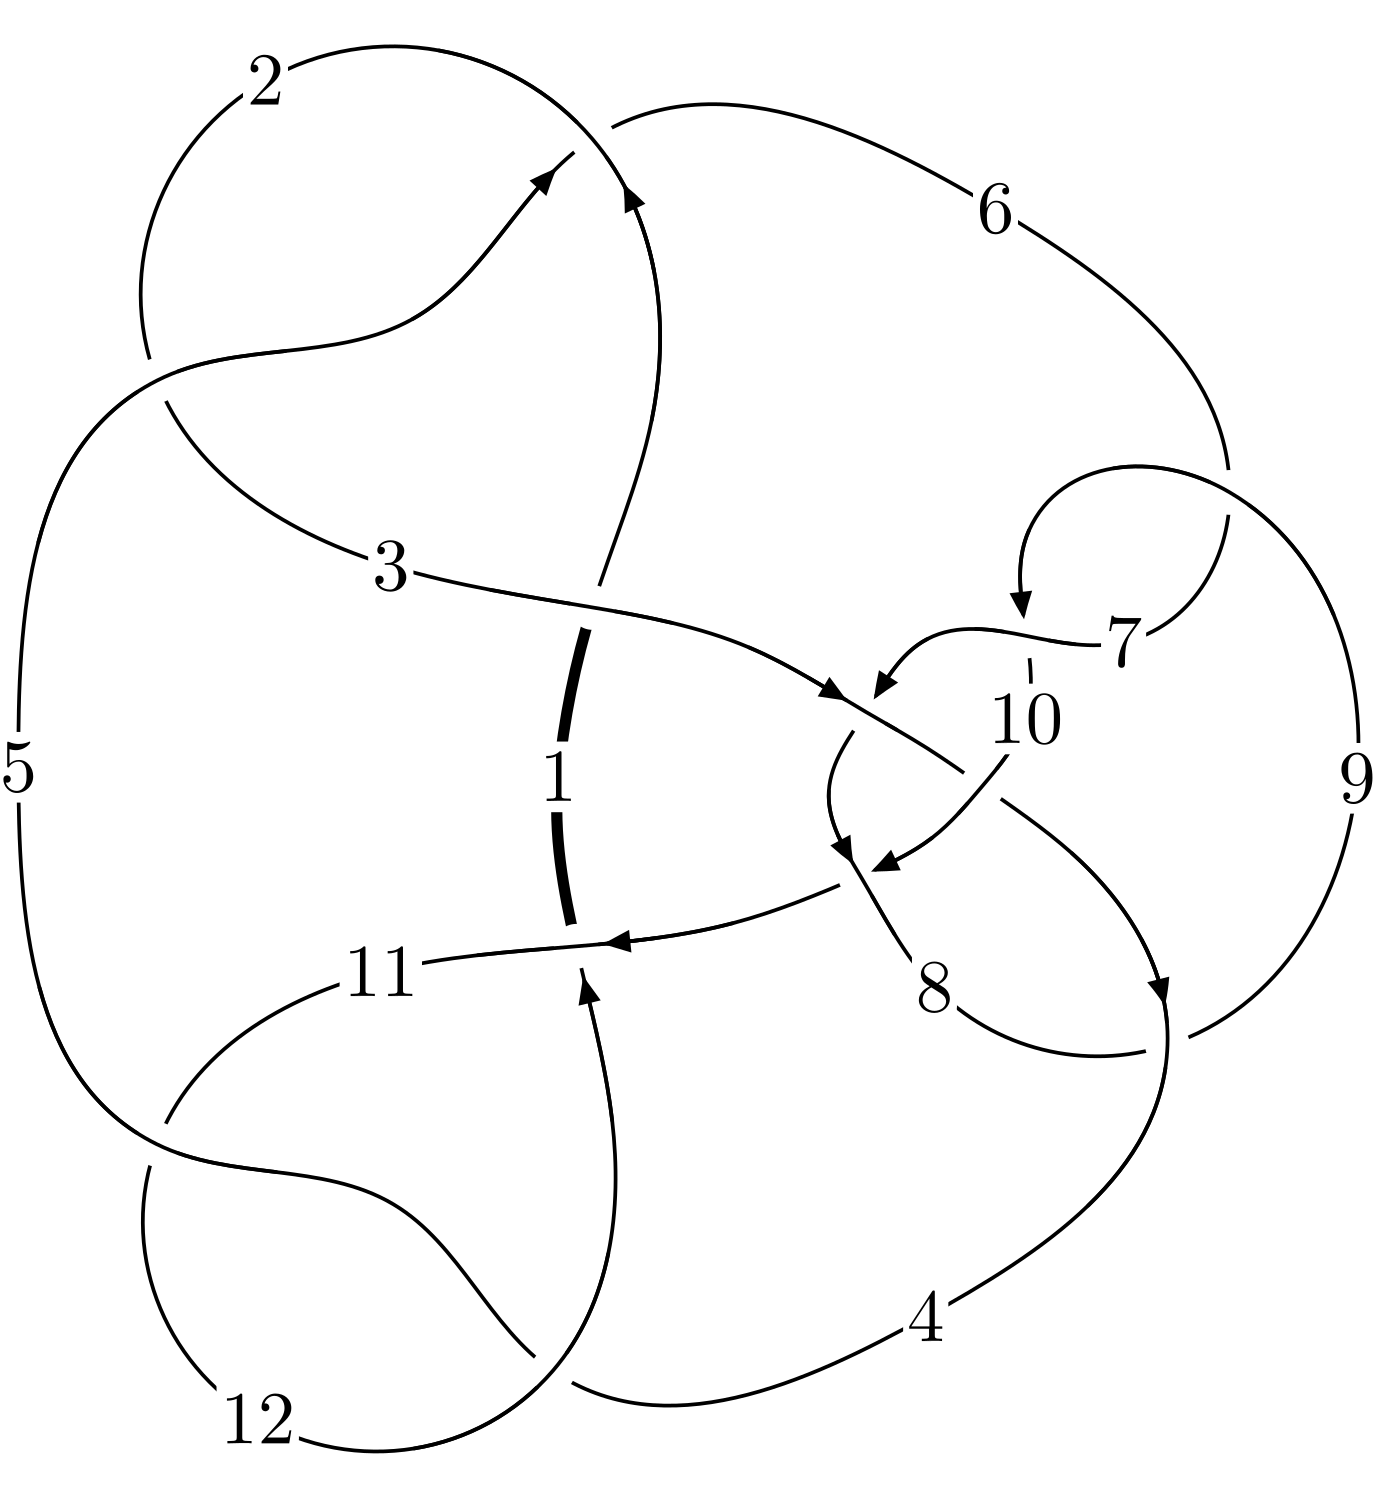
\includegraphics[width=112pt]{../../../GIT/diagram.site/Diagrams/png/2453_12n_0364.png}\\
\ \ \ A knot diagram\footnotemark}&
\allowdisplaybreaks
\textbf{Linearized knot diagam} \\
\cline{2-2}
 &
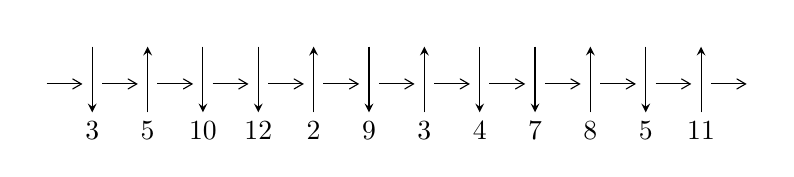
\begin{tikzpicture}[x=20pt, y=17pt]
	% nodes
	\node (C0) at (0, 0) {};
	\node (C1) at (1, 0) {};
	\node (C1U) at (1, +1) {};
	\node (C1D) at (1, -1) {3};

	\node (C2) at (2, 0) {};
	\node (C2U) at (2, +1) {};
	\node (C2D) at (2, -1) {5};

	\node (C3) at (3, 0) {};
	\node (C3U) at (3, +1) {};
	\node (C3D) at (3, -1) {10};

	\node (C4) at (4, 0) {};
	\node (C4U) at (4, +1) {};
	\node (C4D) at (4, -1) {12};

	\node (C5) at (5, 0) {};
	\node (C5U) at (5, +1) {};
	\node (C5D) at (5, -1) {2};

	\node (C6) at (6, 0) {};
	\node (C6U) at (6, +1) {};
	\node (C6D) at (6, -1) {9};

	\node (C7) at (7, 0) {};
	\node (C7U) at (7, +1) {};
	\node (C7D) at (7, -1) {3};

	\node (C8) at (8, 0) {};
	\node (C8U) at (8, +1) {};
	\node (C8D) at (8, -1) {4};

	\node (C9) at (9, 0) {};
	\node (C9U) at (9, +1) {};
	\node (C9D) at (9, -1) {7};

	\node (C10) at (10, 0) {};
	\node (C10U) at (10, +1) {};
	\node (C10D) at (10, -1) {8};

	\node (C11) at (11, 0) {};
	\node (C11U) at (11, +1) {};
	\node (C11D) at (11, -1) {5};

	\node (C12) at (12, 0) {};
	\node (C12U) at (12, +1) {};
	\node (C12D) at (12, -1) {11};
	\node (C13) at (13, 0) {};

	% arrows
	\draw[->,>={angle 60}]
	(C0) edge (C1) (C1) edge (C2) (C2) edge (C3) (C3) edge (C4) (C4) edge (C5) (C5) edge (C6) (C6) edge (C7) (C7) edge (C8) (C8) edge (C9) (C9) edge (C10) (C10) edge (C11) (C11) edge (C12) (C12) edge (C13) ;	\draw[->,>=stealth]
	(C1U) edge (C1D) (C2D) edge (C2U) (C3U) edge (C3D) (C4U) edge (C4D) (C5D) edge (C5U) (C6U) edge (C6D) (C7D) edge (C7U) (C8U) edge (C8D) (C9U) edge (C9D) (C10D) edge (C10U) (C11U) edge (C11D) (C12D) edge (C12U) ;
	\end{tikzpicture} \\
\hhline{~~} \\& 
\textbf{Solving Sequence} \\ \cline{2-2} 
 &
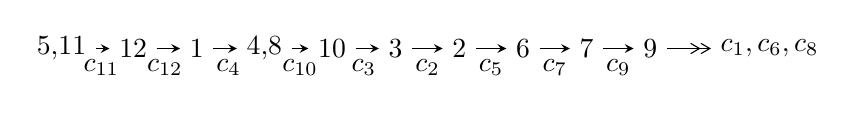
\begin{tikzpicture}[x=23pt, y=7pt]
	% node
	\node (A0) at (-1/8, 0) {5,11};
	\node (A1) at (1, 0) {12};
	\node (A2) at (2, 0) {1};
	\node (A3) at (49/16, 0) {4,8};
	\node (A4) at (33/8, 0) {10};
	\node (A5) at (41/8, 0) {3};
	\node (A6) at (49/8, 0) {2};
	\node (A7) at (57/8, 0) {6};
	\node (A8) at (65/8, 0) {7};
	\node (A9) at (73/8, 0) {9};
	\node (C1) at (1/2, -1) {$c_{11}$};
	\node (C2) at (3/2, -1) {$c_{12}$};
	\node (C3) at (5/2, -1) {$c_{4}$};
	\node (C4) at (29/8, -1) {$c_{10}$};
	\node (C5) at (37/8, -1) {$c_{3}$};
	\node (C6) at (45/8, -1) {$c_{2}$};
	\node (C7) at (53/8, -1) {$c_{5}$};
	\node (C8) at (61/8, -1) {$c_{7}$};
	\node (C9) at (69/8, -1) {$c_{9}$};
	\node (A10) at (11, 0) {$c_{1},c_{6},c_{8}$};

	% edge
	\draw[->,>=stealth]	
	(A0) edge (A1) (A1) edge (A2) (A2) edge (A3) (A3) edge (A4) (A4) edge (A5) (A5) edge (A6) (A6) edge (A7) (A7) edge (A8) (A8) edge (A9) ;
	\draw[->>,>={angle 60}]	
	(A9) edge (A10);
\end{tikzpicture} \\ 

\end{tabular} \\

\footnotetext{
The image of knot diagram is generated by the software ``\textbf{Draw programme}" developed by Andrew Bartholomew(\url{http://www.layer8.co.uk/maths/draw/index.htm\#Running-draw}), where we modified some parts for our purpose(\url{https://github.com/CATsTAILs/LinksPainter}).
}\phantom \\ \newline 
\centering \textbf{Ideals for irreducible components\footnotemark of $X_{\text{par}}$} 
 
\begin{align*}
I^u_{1}&=\langle 
1.65018\times10^{76} u^{49}-3.54268\times10^{76} u^{48}+\cdots+4.05963\times10^{77} b-6.66248\times10^{77},\\
\phantom{I^u_{1}}&\phantom{= \langle  }-6.81584\times10^{77} u^{49}+7.40970\times10^{76} u^{48}+\cdots+1.10422\times10^{80} a-9.55385\times10^{79},\\
\phantom{I^u_{1}}&\phantom{= \langle  }u^{50}-2 u^{49}+\cdots-44 u+17\rangle \\
I^u_{2}&=\langle 
-6839 a^5 u-100530 a^4 u+\cdots-679911 a+101996,\\
\phantom{I^u_{2}}&\phantom{= \langle  }a^6-5 a^5 u-6 a^5+20 a^4 u+2 a^4-16 a^3 u+22 a^3-6 a^2 u-29 a^2+8 a u+7 a- u,\;u^2+1\rangle \\
I^u_{3}&=\langle 
6 u^{12}+24 u^{10}+3 u^9+36 u^8+9 u^7+62 u^6+9 u^5+82 u^4+42 u^3+38 u^2+29 b+39 u+4,\\
\phantom{I^u_{3}}&\phantom{= \langle  }4 u^{13}-22 u^{12}+\cdots+29 a-92,\\
\phantom{I^u_{3}}&\phantom{= \langle  }u^{15}+5 u^{13}- u^{12}+10 u^{11}-4 u^{10}+18 u^9-6 u^8+29 u^7-7 u^6+25 u^5-7 u^4+11 u^3-3 u^2+3 u-1\rangle \\
I^u_{4}&=\langle 
b,\;-3 u^3-2 u^2+4 a-7 u-7,\;u^4- u^3+3 u^2-2 u+1\rangle \\
\\
\end{align*}
\raggedright * 4 irreducible components of $\dim_{\mathbb{C}}=0$, with total 81 representations.\\
\footnotetext{All coefficients of polynomials are rational numbers. But the coefficients are sometimes approximated in decimal forms when there is not enough margin.}
\newpage
\renewcommand{\arraystretch}{1}
\centering \section*{I. $I^u_{1}= \langle 1.65\times10^{76} u^{49}-3.54\times10^{76} u^{48}+\cdots+4.06\times10^{77} b-6.66\times10^{77},\;-6.82\times10^{77} u^{49}+7.41\times10^{76} u^{48}+\cdots+1.10\times10^{80} a-9.55\times10^{79},\;u^{50}-2 u^{49}+\cdots-44 u+17 \rangle$}
\flushleft \textbf{(i) Arc colorings}\\
\begin{tabular}{m{7pt} m{180pt} m{7pt} m{180pt} }
\flushright $a_{5}=$&$\begin{pmatrix}0\\u\end{pmatrix}$ \\
\flushright $a_{11}=$&$\begin{pmatrix}1\\0\end{pmatrix}$ \\
\flushright $a_{12}=$&$\begin{pmatrix}1\\u^2\end{pmatrix}$ \\
\flushright $a_{1}=$&$\begin{pmatrix}u^2+1\\u^2\end{pmatrix}$ \\
\flushright $a_{4}=$&$\begin{pmatrix}u\\u^3+u\end{pmatrix}$ \\
\flushright $a_{8}=$&$\begin{pmatrix}0.00617254 u^{49}-0.000671034 u^{48}+\cdots-2.01092 u+0.865212\\-0.0406485 u^{49}+0.0872659 u^{48}+\cdots-5.79426 u+1.64115\end{pmatrix}$ \\
\flushright $a_{10}=$&$\begin{pmatrix}-0.0282098 u^{49}+0.0868361 u^{48}+\cdots-8.88364 u+0.883519\\-0.0345582 u^{49}+0.0421933 u^{48}+\cdots+0.600393 u-0.0303720\end{pmatrix}$ \\
\flushright $a_{3}=$&$\begin{pmatrix}0.0506811 u^{49}-0.0563455 u^{48}+\cdots+2.97171 u-2.07332\\0.0131686 u^{49}-0.0624266 u^{48}+\cdots+4.05011 u-1.14409\end{pmatrix}$ \\
\flushright $a_{2}=$&$\begin{pmatrix}0.0506811 u^{49}-0.0563455 u^{48}+\cdots+2.97171 u-2.07332\\0.0188729 u^{49}-0.0895465 u^{48}+\cdots+5.16927 u-1.90937\end{pmatrix}$ \\
\flushright $a_{6}=$&$\begin{pmatrix}0.0138068 u^{49}-0.0333179 u^{48}+\cdots+11.0786 u-1.72666\\0.0968175 u^{49}-0.183692 u^{48}+\cdots+0.235614 u-0.540740\end{pmatrix}$ \\
\flushright $a_{7}=$&$\begin{pmatrix}-0.0145850 u^{49}+0.0659148 u^{48}+\cdots-7.07269 u+2.34119\\-0.00275585 u^{49}-0.0265966 u^{48}+\cdots+6.09637 u-1.52987\end{pmatrix}$ \\
\flushright $a_{9}=$&$\begin{pmatrix}0.0367912 u^{49}-0.0525595 u^{48}+\cdots-2.24087 u+0.402118\\-0.0284670 u^{49}+0.0549091 u^{48}+\cdots-6.13338 u+1.01913\end{pmatrix}$\\&\end{tabular}
\flushleft \textbf{(ii) Obstruction class $= -1$}\\~\\
\flushleft \textbf{(iii) Cusp Shapes $= 0.692160 u^{49}-1.33300 u^{48}+\cdots+22.8194 u-11.6257$}\\~\\
\newpage\renewcommand{\arraystretch}{1}
\flushleft \textbf{(iv) u-Polynomials at the component}\newline \\
\begin{tabular}{m{50pt}|m{274pt}}
Crossings & \hspace{64pt}u-Polynomials at each crossing \\
\hline $$\begin{aligned}c_{1}\end{aligned}$$&$\begin{aligned}
&u^{50}+62 u^{49}+\cdots-11952 u+289
\end{aligned}$\\
\hline $$\begin{aligned}c_{2},c_{5}\end{aligned}$$&$\begin{aligned}
&u^{50}+2 u^{49}+\cdots+152 u+17
\end{aligned}$\\
\hline $$\begin{aligned}c_{3}\end{aligned}$$&$\begin{aligned}
&u^{50}-7 u^{49}+\cdots-8 u+4
\end{aligned}$\\
\hline $$\begin{aligned}c_{4},c_{11}\end{aligned}$$&$\begin{aligned}
&u^{50}+2 u^{49}+\cdots+44 u+17
\end{aligned}$\\
\hline $$\begin{aligned}c_{6},c_{9}\end{aligned}$$&$\begin{aligned}
&u^{50}-4 u^{49}+\cdots+127 u+16
\end{aligned}$\\
\hline $$\begin{aligned}c_{7}\end{aligned}$$&$\begin{aligned}
&2(2 u^{50}-3 u^{49}+\cdots-2699 u+3982)
\end{aligned}$\\
\hline $$\begin{aligned}c_{8}\end{aligned}$$&$\begin{aligned}
&2(2 u^{50}+5 u^{49}+\cdots+2584919 u+1407026)
\end{aligned}$\\
\hline $$\begin{aligned}c_{10}\end{aligned}$$&$\begin{aligned}
&u^{50}+8 u^{49}+\cdots-2976 u+256
\end{aligned}$\\
\hline $$\begin{aligned}c_{12}\end{aligned}$$&$\begin{aligned}
&u^{50}-14 u^{49}+\cdots-5136 u+289
\end{aligned}$\\
\hline
\end{tabular}\\~\\
\newpage\renewcommand{\arraystretch}{1}
\flushleft \textbf{(v) Riley Polynomials at the component}\newline \\
\begin{tabular}{m{50pt}|m{274pt}}
Crossings & \hspace{64pt}Riley Polynomials at each crossing \\
\hline $$\begin{aligned}c_{1}\end{aligned}$$&$\begin{aligned}
&y^{50}-134 y^{49}+\cdots-132056732 y+83521
\end{aligned}$\\
\hline $$\begin{aligned}c_{2},c_{5}\end{aligned}$$&$\begin{aligned}
&y^{50}+62 y^{49}+\cdots-11952 y+289
\end{aligned}$\\
\hline $$\begin{aligned}c_{3}\end{aligned}$$&$\begin{aligned}
&y^{50}+y^{49}+\cdots+152 y+16
\end{aligned}$\\
\hline $$\begin{aligned}c_{4},c_{11}\end{aligned}$$&$\begin{aligned}
&y^{50}+14 y^{49}+\cdots+5136 y+289
\end{aligned}$\\
\hline $$\begin{aligned}c_{6},c_{9}\end{aligned}$$&$\begin{aligned}
&y^{50}-40 y^{49}+\cdots+17759 y+256
\end{aligned}$\\
\hline $$\begin{aligned}c_{7}\end{aligned}$$&$\begin{aligned}
&4(4 y^{50}+275 y^{49}+\cdots+6.39567\times10^{8} y+1.58563\times10^{7})
\end{aligned}$\\
\hline $$\begin{aligned}c_{8}\end{aligned}$$&$\begin{aligned}
&4(4 y^{50}+115 y^{49}+\cdots+2.59259\times10^{12} y+1.97972\times10^{12})
\end{aligned}$\\
\hline $$\begin{aligned}c_{10}\end{aligned}$$&$\begin{aligned}
&y^{50}+12 y^{49}+\cdots-1020928 y+65536
\end{aligned}$\\
\hline $$\begin{aligned}c_{12}\end{aligned}$$&$\begin{aligned}
&y^{50}+58 y^{49}+\cdots+8224052 y+83521
\end{aligned}$\\
\hline
\end{tabular}\\~\\
\newpage\flushleft \textbf{(vi) Complex Volumes and Cusp Shapes}
$$\begin{array}{c|c|c}  
\text{Solutions to }I^u_{1}& \I (\text{vol} + \sqrt{-1}CS) & \text{Cusp shape}\\
 \hline 
\begin{aligned}
u &= -0.068272 + 1.028420 I \\
a &= -0.309956 + 0.515004 I \\
b &= \phantom{-}1.003440 - 0.398879 I\end{aligned}
 & \phantom{-}3.59031 - 0.96879 I & \phantom{-}7.50173 + 1.09095 I \\ \hline\begin{aligned}
u &= -0.068272 - 1.028420 I \\
a &= -0.309956 - 0.515004 I \\
b &= \phantom{-}1.003440 + 0.398879 I\end{aligned}
 & \phantom{-}3.59031 + 0.96879 I & \phantom{-}7.50173 - 1.09095 I \\ \hline\begin{aligned}
u &= \phantom{-}0.480788 + 0.815784 I \\
a &= \phantom{-}1.12478 + 0.91870 I \\
b &= -0.158097 + 0.480865 I\end{aligned}
 & \phantom{-}0.01643 - 1.94498 I & -0.87974 + 3.02972 I \\ \hline\begin{aligned}
u &= \phantom{-}0.480788 - 0.815784 I \\
a &= \phantom{-}1.12478 - 0.91870 I \\
b &= -0.158097 - 0.480865 I\end{aligned}
 & \phantom{-}0.01643 + 1.94498 I & -0.87974 - 3.02972 I \\ \hline\begin{aligned}
u &= -0.636460 + 0.850925 I \\
a &= -0.41580 + 1.74505 I \\
b &= \phantom{-}0.83688 + 1.30980 I\end{aligned}
 & \phantom{-}0.03524 + 5.80828 I & -1.80389 - 9.34928 I \\ \hline\begin{aligned}
u &= -0.636460 - 0.850925 I \\
a &= -0.41580 - 1.74505 I \\
b &= \phantom{-}0.83688 - 1.30980 I\end{aligned}
 & \phantom{-}0.03524 - 5.80828 I & -1.80389 + 9.34928 I \\ \hline\begin{aligned}
u &= \phantom{-}0.039464 + 1.141930 I \\
a &= \phantom{-}0.518130 - 0.112235 I \\
b &= -0.960838 + 0.591042 I\end{aligned}
 & \phantom{-}1.43606 - 5.46886 I & \phantom{-}3.64987 + 5.42308 I \\ \hline\begin{aligned}
u &= \phantom{-}0.039464 - 1.141930 I \\
a &= \phantom{-}0.518130 + 0.112235 I \\
b &= -0.960838 - 0.591042 I\end{aligned}
 & \phantom{-}1.43606 + 5.46886 I & \phantom{-}3.64987 - 5.42308 I \\ \hline\begin{aligned}
u &= -0.591483 + 0.619229 I \\
a &= -0.901275 + 0.820990 I \\
b &= -1.25745 + 0.91387 I\end{aligned}
 & -3.72647 + 3.16916 I & -9.86538 - 6.96751 I \\ \hline\begin{aligned}
u &= -0.591483 - 0.619229 I \\
a &= -0.901275 - 0.820990 I \\
b &= -1.25745 - 0.91387 I\end{aligned}
 & -3.72647 - 3.16916 I & -9.86538 + 6.96751 I\\
 \hline 
 \end{array}$$\newpage$$\begin{array}{c|c|c}  
\text{Solutions to }I^u_{1}& \I (\text{vol} + \sqrt{-1}CS) & \text{Cusp shape}\\
 \hline 
\begin{aligned}
u &= -0.914944 + 0.798812 I \\
a &= -0.044773 + 0.967248 I \\
b &= -0.187772 + 0.921101 I\end{aligned}
 & -7.51460 + 1.56660 I & \phantom{-0.000000 } 0. - 4.59872 I \\ \hline\begin{aligned}
u &= -0.914944 - 0.798812 I \\
a &= -0.044773 - 0.967248 I \\
b &= -0.187772 - 0.921101 I\end{aligned}
 & -7.51460 - 1.56660 I & \phantom{-0.000000 -}0. + 4.59872 I \\ \hline\begin{aligned}
u &= \phantom{-}0.114923 + 0.775485 I \\
a &= \phantom{-}1.67601 - 1.41606 I \\
b &= -0.095714 - 0.666726 I\end{aligned}
 & -0.522597 - 1.281740 I & -1.45542 + 3.17634 I \\ \hline\begin{aligned}
u &= \phantom{-}0.114923 - 0.775485 I \\
a &= \phantom{-}1.67601 + 1.41606 I \\
b &= -0.095714 + 0.666726 I\end{aligned}
 & -0.522597 + 1.281740 I & -1.45542 - 3.17634 I \\ \hline\begin{aligned}
u &= \phantom{-}0.391145 + 0.663226 I \\
a &= -5.02638 + 0.41948 I \\
b &= \phantom{-}0.290024 + 0.026703 I\end{aligned}
 & -1.64557 - 1.46182 I & \phantom{-}49.4938 - 3.8392 I \\ \hline\begin{aligned}
u &= \phantom{-}0.391145 - 0.663226 I \\
a &= -5.02638 - 0.41948 I \\
b &= \phantom{-}0.290024 - 0.026703 I\end{aligned}
 & -1.64557 + 1.46182 I & \phantom{-}49.4938 + 3.8392 I \\ \hline\begin{aligned}
u &= \phantom{-}1.016150 + 0.749484 I \\
a &= \phantom{-}0.920704 + 0.734457 I \\
b &= \phantom{-}0.91099 + 1.89793 I\end{aligned}
 & -8.27324 + 2.71933 I & \phantom{-0.000000 } 0 \\ \hline\begin{aligned}
u &= \phantom{-}1.016150 - 0.749484 I \\
a &= \phantom{-}0.920704 - 0.734457 I \\
b &= \phantom{-}0.91099 - 1.89793 I\end{aligned}
 & -8.27324 - 2.71933 I & \phantom{-0.000000 } 0 \\ \hline\begin{aligned}
u &= -0.914753 + 0.943767 I \\
a &= -1.186270 - 0.030672 I \\
b &= \phantom{-}0.806454 - 0.159713 I\end{aligned}
 & -9.24524 + 3.37020 I & \phantom{-0.000000 } 0 \\ \hline\begin{aligned}
u &= -0.914753 - 0.943767 I \\
a &= -1.186270 + 0.030672 I \\
b &= \phantom{-}0.806454 + 0.159713 I\end{aligned}
 & -9.24524 - 3.37020 I & \phantom{-0.000000 } 0\\
 \hline 
 \end{array}$$\newpage$$\begin{array}{c|c|c}  
\text{Solutions to }I^u_{1}& \I (\text{vol} + \sqrt{-1}CS) & \text{Cusp shape}\\
 \hline 
\begin{aligned}
u &= -0.814625 + 1.036590 I \\
a &= \phantom{-}0.774534 - 0.946809 I \\
b &= -0.507417 - 0.813843 I\end{aligned}
 & -6.75526 + 4.85770 I & \phantom{-0.000000 } 0 \\ \hline\begin{aligned}
u &= -0.814625 - 1.036590 I \\
a &= \phantom{-}0.774534 + 0.946809 I \\
b &= -0.507417 + 0.813843 I\end{aligned}
 & -6.75526 - 4.85770 I & \phantom{-0.000000 } 0 \\ \hline\begin{aligned}
u &= -0.870996 + 1.028870 I \\
a &= \phantom{-}0.45821 - 1.35144 I \\
b &= -0.89846 - 1.26634 I\end{aligned}
 & -5.33295 + 11.18530 I & \phantom{-0.000000 } 0 \\ \hline\begin{aligned}
u &= -0.870996 - 1.028870 I \\
a &= \phantom{-}0.45821 + 1.35144 I \\
b &= -0.89846 + 1.26634 I\end{aligned}
 & -5.33295 - 11.18530 I & \phantom{-0.000000 } 0 \\ \hline\begin{aligned}
u &= \phantom{-}1.009310 + 0.913920 I \\
a &= \phantom{-}0.34174 + 1.43865 I \\
b &= -1.96655 + 1.31397 I\end{aligned}
 & -12.29170 - 1.16111 I & \phantom{-0.000000 } 0 \\ \hline\begin{aligned}
u &= \phantom{-}1.009310 - 0.913920 I \\
a &= \phantom{-}0.34174 - 1.43865 I \\
b &= -1.96655 - 1.31397 I\end{aligned}
 & -12.29170 + 1.16111 I & \phantom{-0.000000 } 0 \\ \hline\begin{aligned}
u &= \phantom{-}1.258650 + 0.560245 I \\
a &= -0.518042 - 0.849518 I \\
b &= -0.98522 - 1.50703 I\end{aligned}
 & -14.6583 + 9.1791 I & \phantom{-0.000000 } 0 \\ \hline\begin{aligned}
u &= \phantom{-}1.258650 - 0.560245 I \\
a &= -0.518042 + 0.849518 I \\
b &= -0.98522 + 1.50703 I\end{aligned}
 & -14.6583 - 9.1791 I & \phantom{-0.000000 } 0 \\ \hline\begin{aligned}
u &= \phantom{-}0.952955 + 1.024640 I \\
a &= -0.865928 - 0.017593 I \\
b &= -1.61238 - 1.73076 I\end{aligned}
 & -11.93760 - 5.99162 I & \phantom{-0.000000 } 0 \\ \hline\begin{aligned}
u &= \phantom{-}0.952955 - 1.024640 I \\
a &= -0.865928 + 0.017593 I \\
b &= -1.61238 + 1.73076 I\end{aligned}
 & -11.93760 + 5.99162 I & \phantom{-0.000000 } 0\\
 \hline 
 \end{array}$$\newpage$$\begin{array}{c|c|c}  
\text{Solutions to }I^u_{1}& \I (\text{vol} + \sqrt{-1}CS) & \text{Cusp shape}\\
 \hline 
\begin{aligned}
u &= \phantom{-}0.851045 + 1.112060 I \\
a &= -0.80295 - 1.35413 I \\
b &= \phantom{-}1.33521 - 1.66319 I\end{aligned}
 & -7.12550 - 9.55838 I & \phantom{-0.000000 } 0 \\ \hline\begin{aligned}
u &= \phantom{-}0.851045 - 1.112060 I \\
a &= -0.80295 + 1.35413 I \\
b &= \phantom{-}1.33521 + 1.66319 I\end{aligned}
 & -7.12550 + 9.55838 I & \phantom{-0.000000 } 0 \\ \hline\begin{aligned}
u &= -1.309460 + 0.524121 I \\
a &= \phantom{-}0.222301 - 0.788694 I \\
b &= \phantom{-}0.262227 - 1.380400 I\end{aligned}
 & -14.2488 - 0.8615 I & \phantom{-0.000000 } 0 \\ \hline\begin{aligned}
u &= -1.309460 - 0.524121 I \\
a &= \phantom{-}0.222301 + 0.788694 I \\
b &= \phantom{-}0.262227 + 1.380400 I\end{aligned}
 & -14.2488 + 0.8615 I & \phantom{-0.000000 } 0 \\ \hline\begin{aligned}
u &= -0.404137 + 0.399130 I \\
a &= -0.80482 - 2.22372 I \\
b &= -0.855653 - 0.987594 I\end{aligned}
 & -3.45702 - 0.25001 I & -11.35059 + 0.24450 I \\ \hline\begin{aligned}
u &= -0.404137 - 0.399130 I \\
a &= -0.80482 + 2.22372 I \\
b &= -0.855653 + 0.987594 I\end{aligned}
 & -3.45702 + 0.25001 I & -11.35059 - 0.24450 I \\ \hline\begin{aligned}
u &= \phantom{-}0.90070 + 1.11853 I \\
a &= -0.589704 - 0.573106 I \\
b &= \phantom{-}0.089569 - 1.060610 I\end{aligned}
 & -4.77019 - 2.61015 I & \phantom{-0.000000 } 0 \\ \hline\begin{aligned}
u &= \phantom{-}0.90070 - 1.11853 I \\
a &= -0.589704 + 0.573106 I \\
b &= \phantom{-}0.089569 + 1.060610 I\end{aligned}
 & -4.77019 + 2.61015 I & \phantom{-0.000000 } 0 \\ \hline\begin{aligned}
u &= \phantom{-}0.250161 + 0.501573 I \\
a &= \phantom{-}1.39564 - 0.73889 I \\
b &= \phantom{-}0.239643 - 0.306301 I\end{aligned}
 & -0.235392 - 1.266680 I & -2.17934 + 5.51042 I \\ \hline\begin{aligned}
u &= \phantom{-}0.250161 - 0.501573 I \\
a &= \phantom{-}1.39564 + 0.73889 I \\
b &= \phantom{-}0.239643 + 0.306301 I\end{aligned}
 & -0.235392 + 1.266680 I & -2.17934 - 5.51042 I\\
 \hline 
 \end{array}$$\newpage$$\begin{array}{c|c|c}  
\text{Solutions to }I^u_{1}& \I (\text{vol} + \sqrt{-1}CS) & \text{Cusp shape}\\
 \hline 
\begin{aligned}
u &= -0.176902 + 0.505057 I \\
a &= \phantom{-}1.72876 - 0.17664 I \\
b &= -1.194380 - 0.508201 I\end{aligned}
 & -1.33404 + 5.95631 I & -8.20112 - 6.23089 I \\ \hline\begin{aligned}
u &= -0.176902 - 0.505057 I \\
a &= \phantom{-}1.72876 + 0.17664 I \\
b &= -1.194380 + 0.508201 I\end{aligned}
 & -1.33404 - 5.95631 I & -8.20112 + 6.23089 I \\ \hline\begin{aligned}
u &= \phantom{-}0.82735 + 1.27724 I \\
a &= \phantom{-}0.84861 + 1.21665 I \\
b &= -1.22043 + 1.35112 I\end{aligned}
 & -12.3391 - 16.5813 I & \phantom{-0.000000 } 0 \\ \hline\begin{aligned}
u &= \phantom{-}0.82735 - 1.27724 I \\
a &= \phantom{-}0.84861 - 1.21665 I \\
b &= -1.22043 - 1.35112 I\end{aligned}
 & -12.3391 + 16.5813 I & \phantom{-0.000000 } 0 \\ \hline\begin{aligned}
u &= \phantom{-}0.14425 + 1.53138 I \\
a &= \phantom{-}0.0056819 - 0.0217967 I \\
b &= \phantom{-}0.336796 + 0.195309 I\end{aligned}
 & \phantom{-}5.21341 - 3.02399 I & \phantom{-0.000000 } 0 \\ \hline\begin{aligned}
u &= \phantom{-}0.14425 - 1.53138 I \\
a &= \phantom{-}0.0056819 + 0.0217967 I \\
b &= \phantom{-}0.336796 - 0.195309 I\end{aligned}
 & \phantom{-}5.21341 + 3.02399 I & \phantom{-0.000000 } 0 \\ \hline\begin{aligned}
u &= -0.84092 + 1.31844 I \\
a &= -0.628284 + 0.707391 I \\
b &= \phantom{-}0.639430 + 1.133170 I\end{aligned}
 & -11.7068 + 8.4623 I & \phantom{-0.000000 } 0 \\ \hline\begin{aligned}
u &= -0.84092 - 1.31844 I \\
a &= -0.628284 - 0.707391 I \\
b &= \phantom{-}0.639430 - 1.133170 I\end{aligned}
 & -11.7068 - 8.4623 I & \phantom{-0.000000 } 0 \\ \hline\begin{aligned}
u &= \phantom{-}0.306063 + 0.264763 I \\
a &= -0.67826 - 2.24848 I \\
b &= \phantom{-}1.149680 + 0.120400 I\end{aligned}
 & \phantom{-}0.168989 + 0.748778 I & -4.44695 + 0.25975 I \\ \hline\begin{aligned}
u &= \phantom{-}0.306063 - 0.264763 I \\
a &= -0.67826 + 2.24848 I \\
b &= \phantom{-}1.149680 - 0.120400 I\end{aligned}
 & \phantom{-}0.168989 - 0.748778 I & -4.44695 - 0.25975 I\\
 \hline 
 \end{array}$$\newpage\newpage\renewcommand{\arraystretch}{1}
\centering \section*{II. $I^u_{2}= \langle -6839 a^{5} u-1.01\times10^{5} a^{4} u+\cdots-6.80\times10^{5} a+1.02\times10^{5},\;-5 a^5 u+20 a^4 u+\cdots-29 a^2+7 a,\;u^2+1 \rangle$}
\flushleft \textbf{(i) Arc colorings}\\
\begin{tabular}{m{7pt} m{180pt} m{7pt} m{180pt} }
\flushright $a_{5}=$&$\begin{pmatrix}0\\u\end{pmatrix}$ \\
\flushright $a_{11}=$&$\begin{pmatrix}1\\0\end{pmatrix}$ \\
\flushright $a_{12}=$&$\begin{pmatrix}1\\-1\end{pmatrix}$ \\
\flushright $a_{1}=$&$\begin{pmatrix}0\\-1\end{pmatrix}$ \\
\flushright $a_{4}=$&$\begin{pmatrix}u\\0\end{pmatrix}$ \\
\flushright $a_{8}=$&$\begin{pmatrix}a\\0.163327 a^{5} u+2.40083 a^{4} u+\cdots+16.2375 a-2.43584\end{pmatrix}$ \\
\flushright $a_{10}=$&$\begin{pmatrix}-0.0197263 a^{5} u+0.856399 a^{4} u+\cdots+3.63150 a+0.836673\\0.0806247 a^{5} u-0.463927 a^{4} u+\cdots-1.15007 a+0.616698\end{pmatrix}$ \\
\flushright $a_{3}=$&$\begin{pmatrix}1\\0.320947 a^{5} u-3.11277 a^{4} u+\cdots-7.63413 a+2.20818\end{pmatrix}$ \\
\flushright $a_{2}=$&$\begin{pmatrix}1\\0.320947 a^{5} u-3.11277 a^{4} u+\cdots-7.63413 a+1.20818\end{pmatrix}$ \\
\flushright $a_{6}=$&$\begin{pmatrix}u\\0.283094 a^{5} u-0.227306 a^{4} u+\cdots+5.61761 a-1.94421\end{pmatrix}$ \\
\flushright $a_{7}=$&$\begin{pmatrix}0.0650539 a^{5} u-2.95016 a^{4} u+\cdots-12.4434 a+2.11490\\0.186540 a^{5} u-2.61663 a^{4} u+\cdots-7.68727 a+0.569914\end{pmatrix}$ \\
\flushright $a_{9}=$&$\begin{pmatrix}0.163327 a^{5} u+2.40083 a^{4} u+\cdots+17.2375 a-2.43584\\0.163327 a^{5} u+2.40083 a^{4} u+\cdots+16.2375 a-2.43584\end{pmatrix}$\\&\end{tabular}
\flushleft \textbf{(ii) Obstruction class $= 1$}\\~\\
\flushleft \textbf{(iii) Cusp Shapes $= -\frac{6556}{41873} a^5 u+\frac{362488}{41873} a^4 u+\cdots+\frac{1586112}{41873} a-\frac{146544}{41873}$}\\~\\
\newpage\renewcommand{\arraystretch}{1}
\flushleft \textbf{(iv) u-Polynomials at the component}\newline \\
\begin{tabular}{m{50pt}|m{274pt}}
Crossings & \hspace{64pt}u-Polynomials at each crossing \\
\hline $$\begin{aligned}c_{1},c_{12}\end{aligned}$$&$\begin{aligned}
&(u-1)^{12}
\end{aligned}$\\
\hline $$\begin{aligned}c_{2},c_{4},c_{5}\\c_{11}\end{aligned}$$&$\begin{aligned}
&(u^2+1)^6
\end{aligned}$\\
\hline $$\begin{aligned}c_{3},c_{7}\end{aligned}$$&$\begin{aligned}
&u^{12}- u^{10}+5 u^8+6 u^4-3 u^2+1
\end{aligned}$\\
\hline $$\begin{aligned}c_{6},c_{10}\end{aligned}$$&$\begin{aligned}
&(u^6+u^5- u^4-2 u^3+u+1)^2
\end{aligned}$\\
\hline $$\begin{aligned}c_{8}\end{aligned}$$&$\begin{aligned}
&u^{12}+3 u^{10}+5 u^8+4 u^6+2 u^4+u^2+1
\end{aligned}$\\
\hline $$\begin{aligned}c_{9}\end{aligned}$$&$\begin{aligned}
&(u^6- u^5- u^4+2 u^3- u+1)^2
\end{aligned}$\\
\hline
\end{tabular}\\~\\
\newpage\renewcommand{\arraystretch}{1}
\flushleft \textbf{(v) Riley Polynomials at the component}\newline \\
\begin{tabular}{m{50pt}|m{274pt}}
Crossings & \hspace{64pt}Riley Polynomials at each crossing \\
\hline $$\begin{aligned}c_{1},c_{12}\end{aligned}$$&$\begin{aligned}
&(y-1)^{12}
\end{aligned}$\\
\hline $$\begin{aligned}c_{2},c_{4},c_{5}\\c_{11}\end{aligned}$$&$\begin{aligned}
&(y+1)^{12}
\end{aligned}$\\
\hline $$\begin{aligned}c_{3},c_{7}\end{aligned}$$&$\begin{aligned}
&(y^6- y^5+5 y^4+6 y^2-3 y+1)^2
\end{aligned}$\\
\hline $$\begin{aligned}c_{6},c_{9},c_{10}\end{aligned}$$&$\begin{aligned}
&(y^6-3 y^5+5 y^4-4 y^3+2 y^2- y+1)^2
\end{aligned}$\\
\hline $$\begin{aligned}c_{8}\end{aligned}$$&$\begin{aligned}
&(y^6+3 y^5+5 y^4+4 y^3+2 y^2+y+1)^2
\end{aligned}$\\
\hline
\end{tabular}\\~\\
\newpage\flushleft \textbf{(vi) Complex Volumes and Cusp Shapes}
$$\begin{array}{c|c|c}  
\text{Solutions to }I^u_{2}& \I (\text{vol} + \sqrt{-1}CS) & \text{Cusp shape}\\
 \hline 
\begin{aligned}
u &= \phantom{-0.000000 -}1.000000 I \\
a &= \phantom{-}1.217590 - 0.251449 I \\
b &= -1.073950 + 0.558752 I\end{aligned}
 & \phantom{-0.000000 } -5.69302 I & -2.00000 + 5.51057 I \\ \hline\begin{aligned}
u &= \phantom{-0.000000 -}1.000000 I \\
a &= -1.010760 + 0.965580 I \\
b &= \phantom{-}1.002190 - 0.295542 I\end{aligned}
 & \phantom{-}1.89061 - 0.92430 I & \phantom{-}1.71672 + 0.79423 I \\ \hline\begin{aligned}
u &= \phantom{-0.000000 -}1.000000 I \\
a &= \phantom{-}0.318306 + 0.177934 I \\
b &= \phantom{-}1.002190 + 0.295542 I\end{aligned}
 & \phantom{-}1.89061 + 0.92430 I & \phantom{-}1.71672 - 0.79423 I \\ \hline\begin{aligned}
u &= \phantom{-0.000000 -}1.000000 I \\
a &= \phantom{-}0.100084 + 0.103550 I \\
b &= -1.073950 - 0.558752 I\end{aligned}
 & \phantom{-0.000000 -}5.69302 I & -2.00000 - 5.51057 I \\ \hline\begin{aligned}
u &= \phantom{-0.000000 -}1.000000 I \\
a &= \phantom{-}2.39185 + 1.23447 I \\
b &= -0.428243 - 0.664531 I\end{aligned}
 & -1.89061 - 0.92430 I & -5.71672 + 0.79423 I \\ \hline\begin{aligned}
u &= \phantom{-0.000000 -}1.000000 I \\
a &= \phantom{-}2.98293 + 2.76991 I \\
b &= -0.428243 + 0.664531 I\end{aligned}
 & -1.89061 + 0.92430 I & -5.71672 - 0.79423 I \\ \hline\begin{aligned}
u &= \phantom{-0.000000 } -1.000000 I \\
a &= \phantom{-}1.217590 + 0.251449 I \\
b &= -1.073950 - 0.558752 I\end{aligned}
 & \phantom{-0.000000 -}5.69302 I & -2.00000 - 5.51057 I \\ \hline\begin{aligned}
u &= \phantom{-0.000000 } -1.000000 I \\
a &= -1.010760 - 0.965580 I \\
b &= \phantom{-}1.002190 + 0.295542 I\end{aligned}
 & \phantom{-}1.89061 + 0.92430 I & \phantom{-}1.71672 - 0.79423 I \\ \hline\begin{aligned}
u &= \phantom{-0.000000 } -1.000000 I \\
a &= \phantom{-}0.318306 - 0.177934 I \\
b &= \phantom{-}1.002190 - 0.295542 I\end{aligned}
 & \phantom{-}1.89061 - 0.92430 I & \phantom{-}1.71672 + 0.79423 I \\ \hline\begin{aligned}
u &= \phantom{-0.000000 } -1.000000 I \\
a &= \phantom{-}0.100084 - 0.103550 I \\
b &= -1.073950 + 0.558752 I\end{aligned}
 & \phantom{-0.000000 } -5.69302 I & -2.00000 + 5.51057 I\\
 \hline 
 \end{array}$$\newpage$$\begin{array}{c|c|c}  
\text{Solutions to }I^u_{2}& \I (\text{vol} + \sqrt{-1}CS) & \text{Cusp shape}\\
 \hline 
\begin{aligned}
u &= \phantom{-0.000000 } -1.000000 I \\
a &= \phantom{-}2.39185 - 1.23447 I \\
b &= -0.428243 + 0.664531 I\end{aligned}
 & -1.89061 + 0.92430 I & -5.71672 - 0.79423 I \\ \hline\begin{aligned}
u &= \phantom{-0.000000 } -1.000000 I \\
a &= \phantom{-}2.98293 - 2.76991 I \\
b &= -0.428243 - 0.664531 I\end{aligned}
 & -1.89061 - 0.92430 I & -5.71672 + 0.79423 I\\
 \hline 
 \end{array}$$\newpage\newpage\renewcommand{\arraystretch}{1}
\centering \section*{III. $I^u_{3}= \langle 6 u^{12}+24 u^{10}+\cdots+29 b+4,\;4 u^{13}-22 u^{12}+\cdots+29 a-92,\;u^{15}+5 u^{13}+\cdots+3 u-1 \rangle$}
\flushleft \textbf{(i) Arc colorings}\\
\begin{tabular}{m{7pt} m{180pt} m{7pt} m{180pt} }
\flushright $a_{5}=$&$\begin{pmatrix}0\\u\end{pmatrix}$ \\
\flushright $a_{11}=$&$\begin{pmatrix}1\\0\end{pmatrix}$ \\
\flushright $a_{12}=$&$\begin{pmatrix}1\\u^2\end{pmatrix}$ \\
\flushright $a_{1}=$&$\begin{pmatrix}u^2+1\\u^2\end{pmatrix}$ \\
\flushright $a_{4}=$&$\begin{pmatrix}u\\u^3+u\end{pmatrix}$ \\
\flushright $a_{8}=$&$\begin{pmatrix}-0.137931 u^{13}+0.758621 u^{12}+\cdots-2.82759 u+3.17241\\-0.206897 u^{12}-0.827586 u^{10}+\cdots-1.34483 u-0.137931\end{pmatrix}$ \\
\flushright $a_{10}=$&$\begin{pmatrix}0.586207 u^{13}-0.586207 u^{12}+\cdots-0.586207 u-0.724138\\0.379310 u^{12}+1.51724 u^{10}+\cdots-1.03448 u+0.586207\end{pmatrix}$ \\
\flushright $a_{3}=$&$\begin{pmatrix}1\\0\end{pmatrix}$ \\
\flushright $a_{2}=$&$\begin{pmatrix}1\\u^2\end{pmatrix}$ \\
\flushright $a_{6}=$&$\begin{pmatrix}u\\u^3+u\end{pmatrix}$ \\
\flushright $a_{7}=$&$\begin{pmatrix}-0.137931 u^{13}+0.965517 u^{12}+\cdots-1.48276 u+3.31034\\-0.206897 u^{12}-0.827586 u^{10}+\cdots-1.34483 u-0.137931\end{pmatrix}$ \\
\flushright $a_{9}=$&$\begin{pmatrix}0.758621 u^{12}+3.03448 u^{10}+\cdots-2.06897 u+3.17241\\- u^3- u\end{pmatrix}$\\&\end{tabular}
\flushleft \textbf{(ii) Obstruction class $= -1$}\\~\\
\flushleft \textbf{(iii) Cusp Shapes $= -\frac{28}{29} u^{12}-\frac{112}{29} u^{10}+\frac{44}{29} u^9-\frac{168}{29} u^8+\frac{132}{29} u^7-\frac{328}{29} u^6+\frac{132}{29} u^5-\frac{460}{29} u^4+\frac{268}{29} u^3-\frac{216}{29} u^2+\frac{224}{29} u-\frac{154}{29}$}\\~\\
\newpage\renewcommand{\arraystretch}{1}
\flushleft \textbf{(iv) u-Polynomials at the component}\newline \\
\begin{tabular}{m{50pt}|m{274pt}}
Crossings & \hspace{64pt}u-Polynomials at each crossing \\
\hline $$\begin{aligned}c_{1}\end{aligned}$$&$\begin{aligned}
&u^{15}+10 u^{14}+\cdots+3 u-1
\end{aligned}$\\
\hline $$\begin{aligned}c_{2},c_{4},c_{5}\\c_{11}\end{aligned}$$&$\begin{aligned}
&u^{15}+5 u^{13}+\cdots+3 u+1
\end{aligned}$\\
\hline $$\begin{aligned}c_{3}\end{aligned}$$&$\begin{aligned}
&(u^5+3 u^4+4 u^3+u^2- u-1)^3
\end{aligned}$\\
\hline $$\begin{aligned}c_{6},c_{8},c_{9}\end{aligned}$$&$\begin{aligned}
&(u^5- u^4-2 u^3+u^2+u+1)^3
\end{aligned}$\\
\hline $$\begin{aligned}c_{7},c_{10}\end{aligned}$$&$\begin{aligned}
&(u^5+u^4+2 u^3+u^2+u+1)^3
\end{aligned}$\\
\hline $$\begin{aligned}c_{12}\end{aligned}$$&$\begin{aligned}
&u^{15}-10 u^{14}+\cdots+3 u+1
\end{aligned}$\\
\hline
\end{tabular}\\~\\
\newpage\renewcommand{\arraystretch}{1}
\flushleft \textbf{(v) Riley Polynomials at the component}\newline \\
\begin{tabular}{m{50pt}|m{274pt}}
Crossings & \hspace{64pt}Riley Polynomials at each crossing \\
\hline $$\begin{aligned}c_{1},c_{12}\end{aligned}$$&$\begin{aligned}
&y^{15}-10 y^{14}+\cdots+95 y-1
\end{aligned}$\\
\hline $$\begin{aligned}c_{2},c_{4},c_{5}\\c_{11}\end{aligned}$$&$\begin{aligned}
&y^{15}+10 y^{14}+\cdots+3 y-1
\end{aligned}$\\
\hline $$\begin{aligned}c_{3}\end{aligned}$$&$\begin{aligned}
&(y^5- y^4+8 y^3-3 y^2+3 y-1)^3
\end{aligned}$\\
\hline $$\begin{aligned}c_{6},c_{8},c_{9}\end{aligned}$$&$\begin{aligned}
&(y^5-5 y^4+8 y^3-3 y^2- y-1)^3
\end{aligned}$\\
\hline $$\begin{aligned}c_{7},c_{10}\end{aligned}$$&$\begin{aligned}
&(y^5+3 y^4+4 y^3+y^2- y-1)^3
\end{aligned}$\\
\hline
\end{tabular}\\~\\
\newpage\flushleft \textbf{(vi) Complex Volumes and Cusp Shapes}
$$\begin{array}{c|c|c}  
\text{Solutions to }I^u_{3}& \I (\text{vol} + \sqrt{-1}CS) & \text{Cusp shape}\\
 \hline 
\begin{aligned}
u &= -0.157313 + 1.036460 I \\
a &= \phantom{-}3.87069 - 2.29859 I \\
b &= -0.766826\phantom{ +0.000000I}\end{aligned}
 & -2.40108\phantom{ +0.000000I} & -3.48114 + 0. I\phantom{ +0.000000I} \\ \hline\begin{aligned}
u &= -0.157313 - 1.036460 I \\
a &= \phantom{-}3.87069 + 2.29859 I \\
b &= -0.766826\phantom{ +0.000000I}\end{aligned}
 & -2.40108\phantom{ +0.000000I} & -3.48114 + 0. I\phantom{ +0.000000I} \\ \hline\begin{aligned}
u &= -0.001127 + 1.228660 I \\
a &= \phantom{-}0.207187 - 1.120700 I \\
b &= \phantom{-}0.339110 + 0.822375 I\end{aligned}
 & -0.32910 + 1.53058 I & -2.51511 - 4.43065 I \\ \hline\begin{aligned}
u &= -0.001127 - 1.228660 I \\
a &= \phantom{-}0.207187 + 1.120700 I \\
b &= \phantom{-}0.339110 - 0.822375 I\end{aligned}
 & -0.32910 - 1.53058 I & -2.51511 + 4.43065 I \\ \hline\begin{aligned}
u &= \phantom{-}1.021430 + 0.758717 I \\
a &= \phantom{-}0.119200 + 1.050670 I \\
b &= -0.455697 + 1.200150 I\end{aligned}
 & -5.87256 - 4.40083 I & -6.74431 + 3.49859 I \\ \hline\begin{aligned}
u &= \phantom{-}1.021430 - 0.758717 I \\
a &= \phantom{-}0.119200 - 1.050670 I \\
b &= -0.455697 - 1.200150 I\end{aligned}
 & -5.87256 + 4.40083 I & -6.74431 - 3.49859 I \\ \hline\begin{aligned}
u &= -0.363053 + 0.617188 I \\
a &= \phantom{-}1.69633 - 1.09818 I \\
b &= \phantom{-}0.339110 - 0.822375 I\end{aligned}
 & -0.32910 - 1.53058 I & -2.51511 + 4.43065 I \\ \hline\begin{aligned}
u &= -0.363053 - 0.617188 I \\
a &= \phantom{-}1.69633 + 1.09818 I \\
b &= \phantom{-}0.339110 + 0.822375 I\end{aligned}
 & -0.32910 + 1.53058 I & -2.51511 - 4.43065 I \\ \hline\begin{aligned}
u &= \phantom{-}0.364180 + 0.611475 I \\
a &= \phantom{-}0.74058 - 1.49061 I \\
b &= \phantom{-}0.339110 - 0.822375 I\end{aligned}
 & -0.32910 - 1.53058 I & -2.51511 + 4.43065 I \\ \hline\begin{aligned}
u &= \phantom{-}0.364180 - 0.611475 I \\
a &= \phantom{-}0.74058 + 1.49061 I \\
b &= \phantom{-}0.339110 + 0.822375 I\end{aligned}
 & -0.32910 + 1.53058 I & -2.51511 - 4.43065 I\\
 \hline 
 \end{array}$$\newpage$$\begin{array}{c|c|c}  
\text{Solutions to }I^u_{3}& \I (\text{vol} + \sqrt{-1}CS) & \text{Cusp shape}\\
 \hline 
\begin{aligned}
u &= -0.975116 + 0.872207 I \\
a &= -0.741792 + 0.660626 I \\
b &= -0.455697 + 1.200150 I\end{aligned}
 & -5.87256 - 4.40083 I & -6.74431 + 3.49859 I \\ \hline\begin{aligned}
u &= -0.975116 - 0.872207 I \\
a &= -0.741792 - 0.660626 I \\
b &= -0.455697 - 1.200150 I\end{aligned}
 & -5.87256 + 4.40083 I & -6.74431 - 3.49859 I \\ \hline\begin{aligned}
u &= -0.04631 + 1.63092 I \\
a &= \phantom{-}0.195775 + 0.184082 I \\
b &= -0.455697 - 1.200150 I\end{aligned}
 & -5.87256 + 4.40083 I & -6.74431 - 3.49859 I \\ \hline\begin{aligned}
u &= -0.04631 - 1.63092 I \\
a &= \phantom{-}0.195775 - 0.184082 I \\
b &= -0.455697 + 1.200150 I\end{aligned}
 & -5.87256 - 4.40083 I & -6.74431 + 3.49859 I \\ \hline\begin{aligned}
u &= \phantom{-}0.314625\phantom{ +0.000000I} \\
a &= \phantom{-}2.82406\phantom{ +0.000000I} \\
b &= -0.766826\phantom{ +0.000000I}\end{aligned}
 & -2.40108\phantom{ +0.000000I} & -3.48110\phantom{ +0.000000I}\\
 \hline 
 \end{array}$$\newpage\newpage\renewcommand{\arraystretch}{1}
\centering \section*{IV. $I^u_{4}= \langle b,\;-3 u^3-2 u^2+4 a-7 u-7,\;u^4- u^3+3 u^2-2 u+1 \rangle$}
\flushleft \textbf{(i) Arc colorings}\\
\begin{tabular}{m{7pt} m{180pt} m{7pt} m{180pt} }
\flushright $a_{5}=$&$\begin{pmatrix}0\\u\end{pmatrix}$ \\
\flushright $a_{11}=$&$\begin{pmatrix}1\\0\end{pmatrix}$ \\
\flushright $a_{12}=$&$\begin{pmatrix}1\\u^2\end{pmatrix}$ \\
\flushright $a_{1}=$&$\begin{pmatrix}u^2+1\\u^2\end{pmatrix}$ \\
\flushright $a_{4}=$&$\begin{pmatrix}u\\u^3+u\end{pmatrix}$ \\
\flushright $a_{8}=$&$\begin{pmatrix}\frac{3}{4} u^3+\frac{1}{2} u^2+\frac{7}{4} u+\frac{7}{4}\\0\end{pmatrix}$ \\
\flushright $a_{10}=$&$\begin{pmatrix}1\\0\end{pmatrix}$ \\
\flushright $a_{3}=$&$\begin{pmatrix}u^3+2 u\\u^3+u\end{pmatrix}$ \\
\flushright $a_{2}=$&$\begin{pmatrix}u^3+2 u\\u^3- u^2+2 u-1\end{pmatrix}$ \\
\flushright $a_{6}=$&$\begin{pmatrix}-1\\0\end{pmatrix}$ \\
\flushright $a_{7}=$&$\begin{pmatrix}\frac{5}{4} u^3-\frac{1}{2} u^2+\frac{13}{4} u-\frac{3}{4}\\-1\end{pmatrix}$ \\
\flushright $a_{9}=$&$\begin{pmatrix}\frac{5}{4} u^3-\frac{1}{2} u^2+\frac{13}{4} u+\frac{1}{4}\\-1\end{pmatrix}$\\&\end{tabular}
\flushleft \textbf{(ii) Obstruction class $= 1$}\\~\\
\flushleft \textbf{(iii) Cusp Shapes $= -\frac{113}{16} u^3+\frac{21}{8} u^2-\frac{13}{16} u-\frac{169}{16}$}\\~\\
\newpage\renewcommand{\arraystretch}{1}
\flushleft \textbf{(iv) u-Polynomials at the component}\newline \\
\begin{tabular}{m{50pt}|m{274pt}}
Crossings & \hspace{64pt}u-Polynomials at each crossing \\
\hline $$\begin{aligned}c_{1},c_{11}\end{aligned}$$&$\begin{aligned}
&u^4- u^3+3 u^2-2 u+1
\end{aligned}$\\
\hline $$\begin{aligned}c_{2}\end{aligned}$$&$\begin{aligned}
&u^4- u^3+u^2+1
\end{aligned}$\\
\hline $$\begin{aligned}c_{3}\end{aligned}$$&$\begin{aligned}
&u^4- u^3+5 u^2+u+2
\end{aligned}$\\
\hline $$\begin{aligned}c_{4}\end{aligned}$$&$\begin{aligned}
&u^4+u^3+3 u^2+2 u+1
\end{aligned}$\\
\hline $$\begin{aligned}c_{5}\end{aligned}$$&$\begin{aligned}
&u^4+u^3+u^2+1
\end{aligned}$\\
\hline $$\begin{aligned}c_{6}\end{aligned}$$&$\begin{aligned}
&(u-1)^4
\end{aligned}$\\
\hline $$\begin{aligned}c_{7},c_{8}\end{aligned}$$&$\begin{aligned}
&2(2 u^4+u^3+5 u^2- u+1)
\end{aligned}$\\
\hline $$\begin{aligned}c_{9}\end{aligned}$$&$\begin{aligned}
&(u+1)^4
\end{aligned}$\\
\hline $$\begin{aligned}c_{10}\end{aligned}$$&$\begin{aligned}
&u^4
\end{aligned}$\\
\hline $$\begin{aligned}c_{12}\end{aligned}$$&$\begin{aligned}
&u^4-5 u^3+7 u^2-2 u+1
\end{aligned}$\\
\hline
\end{tabular}\\~\\
\newpage\renewcommand{\arraystretch}{1}
\flushleft \textbf{(v) Riley Polynomials at the component}\newline \\
\begin{tabular}{m{50pt}|m{274pt}}
Crossings & \hspace{64pt}Riley Polynomials at each crossing \\
\hline $$\begin{aligned}c_{1},c_{4},c_{11}\end{aligned}$$&$\begin{aligned}
&y^4+5 y^3+7 y^2+2 y+1
\end{aligned}$\\
\hline $$\begin{aligned}c_{2},c_{5}\end{aligned}$$&$\begin{aligned}
&y^4+y^3+3 y^2+2 y+1
\end{aligned}$\\
\hline $$\begin{aligned}c_{3}\end{aligned}$$&$\begin{aligned}
&y^4+9 y^3+31 y^2+19 y+4
\end{aligned}$\\
\hline $$\begin{aligned}c_{6},c_{9}\end{aligned}$$&$\begin{aligned}
&(y-1)^4
\end{aligned}$\\
\hline $$\begin{aligned}c_{7},c_{8}\end{aligned}$$&$\begin{aligned}
&4(4 y^4+19 y^3+31 y^2+9 y+1)
\end{aligned}$\\
\hline $$\begin{aligned}c_{10}\end{aligned}$$&$\begin{aligned}
&y^4
\end{aligned}$\\
\hline $$\begin{aligned}c_{12}\end{aligned}$$&$\begin{aligned}
&y^4-11 y^3+31 y^2+10 y+1
\end{aligned}$\\
\hline
\end{tabular}\\~\\
\newpage\flushleft \textbf{(vi) Complex Volumes and Cusp Shapes}
$$\begin{array}{c|c|c}  
\text{Solutions to }I^u_{4}& \I (\text{vol} + \sqrt{-1}CS) & \text{Cusp shape}\\
 \hline 
\begin{aligned}
u &= \phantom{-}0.395123 + 0.506844 I \\
a &= \phantom{-}2.20896 + 1.16763 I \\
b &= \phantom{-0.000000 } 0\end{aligned}
 & -1.85594 - 1.41510 I & -9.43312 - 0.11741 I \\ \hline\begin{aligned}
u &= \phantom{-}0.395123 - 0.506844 I \\
a &= \phantom{-}2.20896 - 1.16763 I \\
b &= \phantom{-0.000000 } 0\end{aligned}
 & -1.85594 + 1.41510 I & -9.43312 + 0.11741 I \\ \hline\begin{aligned}
u &= \phantom{-}0.10488 + 1.55249 I \\
a &= \phantom{-}0.166035 + 0.111704 I \\
b &= \phantom{-0.000000 } 0\end{aligned}
 & \phantom{-}5.14581 - 3.16396 I & -11.5981 + 25.6585 I \\ \hline\begin{aligned}
u &= \phantom{-}0.10488 - 1.55249 I \\
a &= \phantom{-}0.166035 - 0.111704 I \\
b &= \phantom{-0.000000 } 0\end{aligned}
 & \phantom{-}5.14581 + 3.16396 I & -11.5981 - 25.6585 I\\
 \hline 
 \end{array}$$\newpage
\newpage\renewcommand{\arraystretch}{1}
\centering \section*{ V. u-Polynomials}
\begin{tabular}{m{50pt}|m{274pt}}
Crossings & \hspace{64pt}u-Polynomials at each crossing \\
\hline $$\begin{aligned}c_{1}\end{aligned}$$&$\begin{aligned}
&((u-1)^{12})(u^4- u^3+3 u^2-2 u+1)(u^{15}+10 u^{14}+\cdots+3 u-1)\\
&\cdot(u^{50}+62 u^{49}+\cdots-11952 u+289)
\end{aligned}$\\
\hline $$\begin{aligned}c_{2}\end{aligned}$$&$\begin{aligned}
&((u^2+1)^6)(u^4- u^3+u^2+1)(u^{15}+5 u^{13}+\cdots+3 u+1)\\
&\cdot(u^{50}+2 u^{49}+\cdots+152 u+17)
\end{aligned}$\\
\hline $$\begin{aligned}c_{3}\end{aligned}$$&$\begin{aligned}
&(u^4- u^3+5 u^2+u+2)(u^5+3 u^4+4 u^3+u^2- u-1)^3\\
&\cdot(u^{12}- u^{10}+5 u^8+6 u^4-3 u^2+1)(u^{50}-7 u^{49}+\cdots-8 u+4)
\end{aligned}$\\
\hline $$\begin{aligned}c_{4}\end{aligned}$$&$\begin{aligned}
&((u^2+1)^6)(u^4+u^3+3 u^2+2 u+1)(u^{15}+5 u^{13}+\cdots+3 u+1)\\
&\cdot(u^{50}+2 u^{49}+\cdots+44 u+17)
\end{aligned}$\\
\hline $$\begin{aligned}c_{5}\end{aligned}$$&$\begin{aligned}
&((u^2+1)^6)(u^4+u^3+u^2+1)(u^{15}+5 u^{13}+\cdots+3 u+1)\\
&\cdot(u^{50}+2 u^{49}+\cdots+152 u+17)
\end{aligned}$\\
\hline $$\begin{aligned}c_{6}\end{aligned}$$&$\begin{aligned}
&(u-1)^4(u^5- u^4-2 u^3+u^2+u+1)^3(u^6+u^5- u^4-2 u^3+u+1)^2\\
&\cdot(u^{50}-4 u^{49}+\cdots+127 u+16)
\end{aligned}$\\
\hline $$\begin{aligned}c_{7}\end{aligned}$$&$\begin{aligned}
&4(2 u^4+u^3+5 u^2- u+1)(u^5+u^4+2 u^3+u^2+u+1)^3\\
&\cdot(u^{12}- u^{10}+5 u^8+6 u^4-3 u^2+1)(2 u^{50}-3 u^{49}+\cdots-2699 u+3982)
\end{aligned}$\\
\hline $$\begin{aligned}c_{8}\end{aligned}$$&$\begin{aligned}
&4(2 u^4+u^3+5 u^2- u+1)(u^5- u^4-2 u^3+u^2+u+1)^3\\
&\cdot(u^{12}+3 u^{10}+5 u^8+4 u^6+2 u^4+u^2+1)\\
&\cdot(2 u^{50}+5 u^{49}+\cdots+2584919 u+1407026)
\end{aligned}$\\
\hline $$\begin{aligned}c_{9}\end{aligned}$$&$\begin{aligned}
&(u+1)^4(u^5- u^4-2 u^3+u^2+u+1)^3(u^6- u^5- u^4+2 u^3- u+1)^2\\
&\cdot(u^{50}-4 u^{49}+\cdots+127 u+16)
\end{aligned}$\\
\hline $$\begin{aligned}c_{10}\end{aligned}$$&$\begin{aligned}
&u^4(u^5+u^4+2 u^3+u^2+u+1)^3(u^6+u^5- u^4-2 u^3+u+1)^2\\
&\cdot(u^{50}+8 u^{49}+\cdots-2976 u+256)
\end{aligned}$\\
\hline $$\begin{aligned}c_{11}\end{aligned}$$&$\begin{aligned}
&((u^2+1)^6)(u^4- u^3+3 u^2-2 u+1)(u^{15}+5 u^{13}+\cdots+3 u+1)\\
&\cdot(u^{50}+2 u^{49}+\cdots+44 u+17)
\end{aligned}$\\
\hline $$\begin{aligned}c_{12}\end{aligned}$$&$\begin{aligned}
&((u-1)^{12})(u^4-5 u^3+\cdots-2 u+1)(u^{15}-10 u^{14}+\cdots+3 u+1)\\
&\cdot(u^{50}-14 u^{49}+\cdots-5136 u+289)
\end{aligned}$\\
\hline
\end{tabular}\newpage\renewcommand{\arraystretch}{1}
\centering \section*{ VI. Riley Polynomials}
\begin{tabular}{m{50pt}|m{274pt}}
Crossings & \hspace{64pt}Riley Polynomials at each crossing \\
\hline $$\begin{aligned}c_{1}\end{aligned}$$&$\begin{aligned}
&((y-1)^{12})(y^4+5 y^3+\cdots+2 y+1)(y^{15}-10 y^{14}+\cdots+95 y-1)\\
&\cdot(y^{50}-134 y^{49}+\cdots-132056732 y+83521)
\end{aligned}$\\
\hline $$\begin{aligned}c_{2},c_{5}\end{aligned}$$&$\begin{aligned}
&((y+1)^{12})(y^4+y^3+3 y^2+2 y+1)(y^{15}+10 y^{14}+\cdots+3 y-1)\\
&\cdot(y^{50}+62 y^{49}+\cdots-11952 y+289)
\end{aligned}$\\
\hline $$\begin{aligned}c_{3}\end{aligned}$$&$\begin{aligned}
&(y^4+9 y^3+31 y^2+19 y+4)(y^5- y^4+8 y^3-3 y^2+3 y-1)^3\\
&\cdot((y^6- y^5+5 y^4+6 y^2-3 y+1)^2)(y^{50}+y^{49}+\cdots+152 y+16)
\end{aligned}$\\
\hline $$\begin{aligned}c_{4},c_{11}\end{aligned}$$&$\begin{aligned}
&((y+1)^{12})(y^4+5 y^3+\cdots+2 y+1)(y^{15}+10 y^{14}+\cdots+3 y-1)\\
&\cdot(y^{50}+14 y^{49}+\cdots+5136 y+289)
\end{aligned}$\\
\hline $$\begin{aligned}c_{6},c_{9}\end{aligned}$$&$\begin{aligned}
&(y-1)^4(y^5-5 y^4+8 y^3-3 y^2- y-1)^3\\
&\cdot(y^6-3 y^5+5 y^4-4 y^3+2 y^2- y+1)^2\\
&\cdot(y^{50}-40 y^{49}+\cdots+17759 y+256)
\end{aligned}$\\
\hline $$\begin{aligned}c_{7}\end{aligned}$$&$\begin{aligned}
&16(4 y^4+19 y^3+31 y^2+9 y+1)(y^5+3 y^4+4 y^3+y^2- y-1)^3\\
&\cdot(y^6- y^5+5 y^4+6 y^2-3 y+1)^2\\
&\cdot(4 y^{50}+275 y^{49}+\cdots+639567407 y+15856324)
\end{aligned}$\\
\hline $$\begin{aligned}c_{8}\end{aligned}$$&$\begin{aligned}
&16(4 y^4+19 y^3+31 y^2+9 y+1)(y^5-5 y^4+8 y^3-3 y^2- y-1)^3\\
&\cdot(y^6+3 y^5+5 y^4+4 y^3+2 y^2+y+1)^2\\
&\cdot(4 y^{50}+115 y^{49}+\cdots+2592594386231 y+1979722164676)
\end{aligned}$\\
\hline $$\begin{aligned}c_{10}\end{aligned}$$&$\begin{aligned}
&y^4(y^5+3 y^4+\cdots- y-1)^{3}(y^6-3 y^5+\cdots- y+1)^{2}\\
&\cdot(y^{50}+12 y^{49}+\cdots-1020928 y+65536)
\end{aligned}$\\
\hline $$\begin{aligned}c_{12}\end{aligned}$$&$\begin{aligned}
&((y-1)^{12})(y^4-11 y^3+\cdots+10 y+1)(y^{15}-10 y^{14}+\cdots+95 y-1)\\
&\cdot(y^{50}+58 y^{49}+\cdots+8224052 y+83521)
\end{aligned}$\\
\hline
\end{tabular}
\vskip 2pc
\end{document}